\section*{RMS/Complex Power/Max Power Transfer} \label{sec:Complex Power}
	\vspace{-6mm}
	\begin{multicols}{2}
		\begin{itemize}[noitemsep]
			\item $X_{rms}=\sqrt{\frac{1}{T} \int_{0}^{T} x(t)^2 dt}=\frac{X_{PP}}{2 \sqrt{2}}=\frac{X_{PP}}{2 \sqrt{2}}$
			\item $P_{avg}=\frac{1}{2} \Re\lbrace \mathbf{V} \mathbf{I}^* \rbrace=\frac{1}{2}V_{m}I_{m}\cos \left(\theta_v -\theta_i \right)$
			\item $\mathbf{S} = I_{rms}^2\mathbf{Z} = \frac{V_{rms}^2}{\mathbf{Z}^*} = \mathbf{V}_{rms}\mathbf{I}_{rms}^*$ \vspace{1.2mm}
			\item $\sum_{k=1}^{n} S_{k}$ \vspace{1.2mm}
			\item $C = \frac{Q_{C}}{\omega V_{rms}^2} = \frac{P\left( \tan \theta_1 - \tan \theta_2 \right)}{\omega V_{rms}^2}$ \vspace{1.2mm}
			\item $L=\frac{V_{rms}^2}{\omega \left(Q_1 - Q_2 \right)}$
		\end{itemize}

		\columnbreak
		
		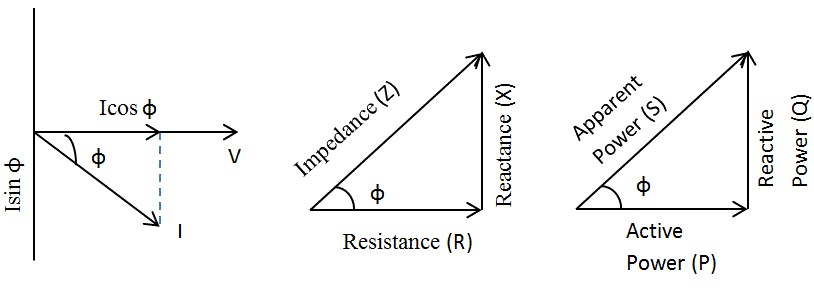
\includegraphics[scale=0.375]{Phasor_Power_Triangle.jpg} % Can't do figure because floats aren't allowed in multicol
		\label{fig:Phasor/Power Triangle}
	\end{multicols}
	\vspace{-4mm}

	\begin{table}[h!] % Complex Power Table
		\centering
		\renewcommand{\arraystretch}{1.4}
		\begin{tabular}{|c|c|c|c|}
			\hline
			\textbf{Name} & \textbf{Symbol} & \textbf{Equation(s)} & \textbf{Units} \\ \hline
			Complex Power & $\mathbf{S}$ & $\frac{P}{Pf} \angle\arccos\left( Pf\right)=P+\jmath Q=\mathbf{V}_{rms} \mathbf{I}_{rms}^{*} = \lvert \mathbf{V}_{rms}\rvert \lvert \mathbf{I}_{rms}\rvert \angle \left( \theta_v - \theta_i\right) $ & \si{\volt \ampere} \\ \hline
			Apparent Power & $S$ & $\lVert \mathbf{S} \rVert = \lvert \mathbf{V}_{rms} \rvert \lvert \mathbf{I}_{rms} \rvert = \sqrt{P^2 + Q^2}$ & \si{\volt \ampere} \\ \hline
			Real Power & $P$ & $\Re\lbrace \mathbf{S} \rbrace = S * Pf \cos \left[ \arccos \left( Pf \right) \right] = S \cos\left( \theta_v - \theta_i \right)$ & \si{\watt} \\ \hline
			Reactive (Imaginary) Power & $Q$ & $\Im\lbrace \mathbf{S} \rbrace = S * Pf \sin \left[ \arccos \left( Pf \right) \right] =  S \sin \left( \theta_v - \theta_i \right)$ & \si{VAR}\\ \hline
			Power Factor &\textit{Pf} & $\frac{P}{S} = \cos(\theta_v - \theta_i)$ & Lead/Lag \\ \hline
		\end{tabular}
	\end{table}
	\textbf{NOTE:} If you are looking for 3-Phase complex power, it is in \nameref{sec:3-Phase}.
	\vspace{-4mm}